\documentclass[crop, tikz]{standalone}
\usepackage{tikz}

\usetikzlibrary{arrows, positioning}

\tikzstyle{block} = [rectangle, draw, fill=blue!20, 
    text width=5em, text centered, rounded corners, minimum height=4em]
\tikzstyle{line} = [draw, -latex']

\definecolor{mygreen}{rgb}{0,0.6,0}
\definecolor{echodrk}{HTML}{0099cc}

\begin{document}
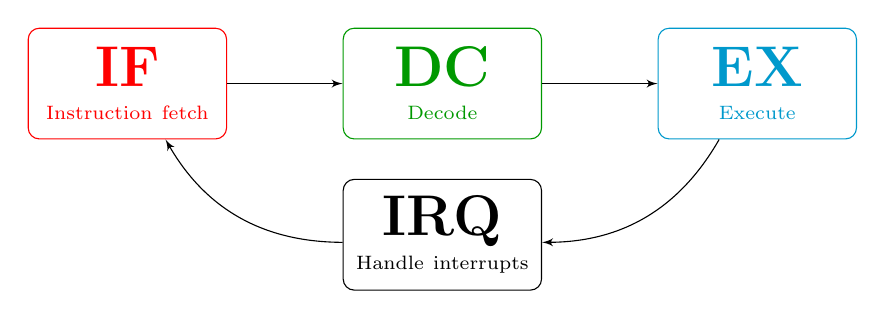
\begin{tikzpicture}[node distance=4cm, auto]
	\node [block, color=red, fill=white, text width=6.5em] (if) {{\huge \bf IF}\\{\scriptsize Instruction fetch}};
	\node [block, color=mygreen, fill=white, text width=6.5em, right of=if] (dc) {{\huge \bf DC}\\{\scriptsize Decode}};
	\node [block, color=echodrk, fill=white, text width=6.5em, right of=dc] (ex) {{\huge \bf EX}\\{\scriptsize Execute}};
	\node [block, color=black, fill=white, text width=6.5em, below = 0.5cm of dc] (intr) {{\huge \bf IRQ}\\{\scriptsize Handle interrupts}};
    
	\path [line] (if) -- (dc);
	\path [line] (dc) -- (ex);
	\path [line] (ex) edge [bend left] (intr);
	\path [line] (intr) edge [bend left] (if);
\end{tikzpicture}
\end{document}
